% -*- mode:LaTex; mode:visual-line; mode:flyspell; fill-column:75-*-

\chapter{Introduction} \label{chap:introduction}

% Introduction.

% \section{Installation instructions}

% This template was tested with TeX Live 2017, which includes all required packages~\cite{TUG2017}. Mac users: this is included as part of OSX and TeXShop. After successfully installing TeX Live, compile the PDF file using your favorite build tool (we tested with \verb!make! on OSX).

% \section{How to use this template}
% Write each chapter as a separate \LaTeX\ file and include them in \verb!thesis-main.tex!. Edit the abstract, acknowledgments, background, title, dedication, and funding files as necessary. Include additional packages in \verb!thesis-packages.tex! and define helpful macros in \verb!thesis-macros.tex!.

% \subsection{Algorithms}
% Define each algorithm as a separate \LaTeX\ file in the algorithms folder using either the \verb!algorithmicx! or \verb!algpseudocode! packages. For example, see Algorithm~\ref{algTemplate}.

% % -*- mode:LaTex; mode:visual-line -*-

\begin{algorithm}
\begin{algorithmic}[1]
\Procedure{Do it}{$N$}
\State Initialize all the things!

\For{t = 1 to N}
\State Do it!
\EndFor
\State \Return $N$
\EndProcedure
\end{algorithmic}
\caption[short caption]{Longer caption}
\label{algTemplate}
\end{algorithm}

\section{SLAM}

Simultaneous Localization and Mapping (SLAM) is the chicken-and-egg problem of estimating the model of the environment (the map), and simultaneously optimizing the robot trajectory associated with the map, given measurements.

Typically, when the map is modeled as a collection of landmarks $ \Lc = \{\ell_m\}_{m=1}^{M} $, and the robot trajectory is modeled as a sequence of poses $\Xc = \{\xv_t\}_{t=1}^{T}$, given a set of measurements $ \Zc = \{\zv_n\}_{n=1}^{N}$, the SLAM problem can be summarized as a maximum-a-posteriori estimation \cite{dellaertFactorGraphsRobot2017} as follows:
\begin{align}
    \hat{\Xc}, \hat{\Lc} &= \argmax_{\Xc, \Lc} p(\Xc, \Lc | \Zc) \\
                         &\propto \argmax_{\Xc, \Lc} p(\Zc | \Xc, \Lc) p(\Xc, \Lc)
\end{align}
Note, that the above problem assumes known \emph{data association} between measurements $\zv_n$ of landmark $\ell_{\beta_n}$ at a robot pose $\xv_{\alpha_n}$as $\Dc := \{(\alpha_n, \beta_n)\}_{n=1}^{N}$ \cite{bowmanProbabilisticDataAssociation2017}.

In reality, however, a SLAM framework for a robot needs to deal with raw sensor measurements. Therefore, typically the system is divided into two parts: \emph{front-end} and \emph{back-end}. The front-end is dedicated to data pre-processing, data association and feeds into the back-end, dedicated to the optimization that results in the best estimate of robot state and landmarks.

\section{Semantics in SLAM}

For autonomous robots in the near future, to work in the real world, advanced interpretation of the environment is necessary. For workloads ranging from semantic 3D reconstruction and path planning, to active interaction with the environment (see Figure~\ref{fig:spot-mini}). These workloads require not only geometric perception including robot localization and map reconstruction, but also semantic and compositional understanding of scenes.

\begin{figure}[htpb]
    \centering
    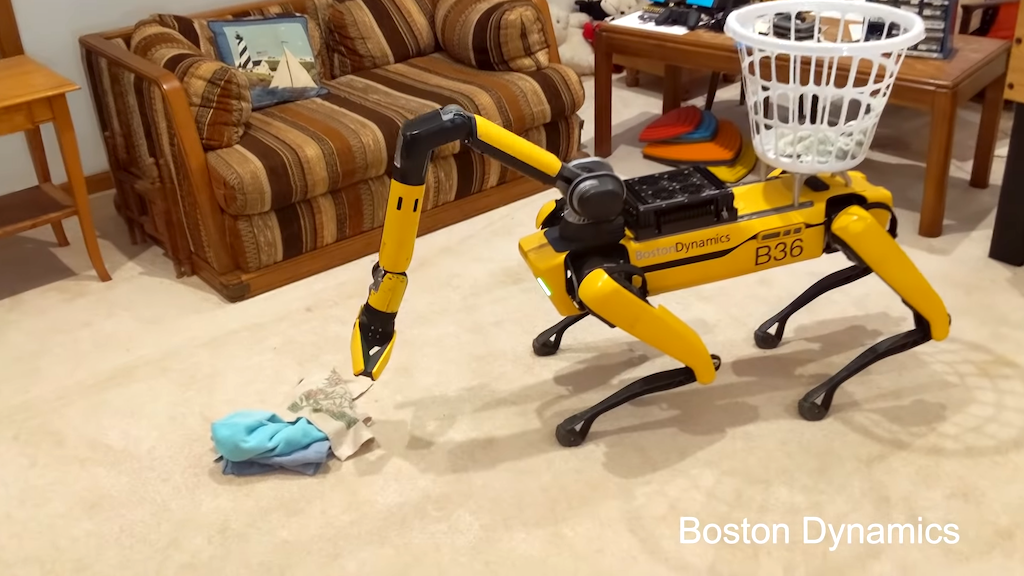
\includegraphics[width=0.8\linewidth]{figs/Spots-Got-an-Arm.png}
    \caption{Boston Dynamics' Spot Mini robot picking up clothes in a living room. These types of complex interactions require the robot to have a semantic understanding of the objects in its environment}%
    \label{fig:spot-mini}
\end{figure}

In recent years, geometry-based SLAM has achieved high levels of performance in \textit{experimental setups} for localization tasks. Many variants of SLAM algorithms, from ORB-SLAM~\cite{mur-artalORBSLAM2OpenSourceSLAM2017} to Direct Sparse Odometry (DSO)~\cite{engelDirectSparseOdometry2018}, can now run in real-time with high trajectory accuracy.
However, they are in general limited by the \emph{static-world} assumption and low-level scene representation as sparse 3D feature points, and thus cannot distill high-level information (semantic understanding) in scenes and adjust to structured environmental changes.

On the other hand, with progress in deep learning, near real-time semantic perception is achievable powered by efficient Deep Neural Networks (DNNs).
Researchers have started to switch to semantic SLAM taking advantage of off-the-shelf solutions; pioneering research includes SLAM++~\cite{salas-morenoSLAMSimultaneousLocalisation2013}, Fusion++~\cite{mccormacFusionVolumetricObjectLevel2018}, and MaskFusion~\cite{runzMaskFusionRealTimeRecognition2018}. These initial attempts take into consideration semantic segmentation, but typically simply attach DNN frontends to existing SLAM frameworks in an ad hoc fashion. Implementation-wise, they require high-end machines to achieve near real-time performance, or are not available to the community.

\section{Thesis}
In this dissertation, I present a Compositional and Scalable Object SLAM system that represents an environment as a posegraph of persistent objects. I describe a system, that incrementally improves each associated persistent object landmarks through RGB-D Fusion, and optimizes the landmarks and the robot trajectory simultaneously to accurately represent an environment. (see Figure~\ref{fig:objectsandscene}).

In implementation, this work fully exploits the power of the modern GPU-based reconstruction pipeline~\cite{dongGPUAcceleratedRobust2019} and object detection frameworks~\cite{kirillovPointRendImageSegmentation2020}, to design an efficient architecture for data exchange without sacrificing the ease of system configuration and build.

\begin{figure}[t!]
    \centering
    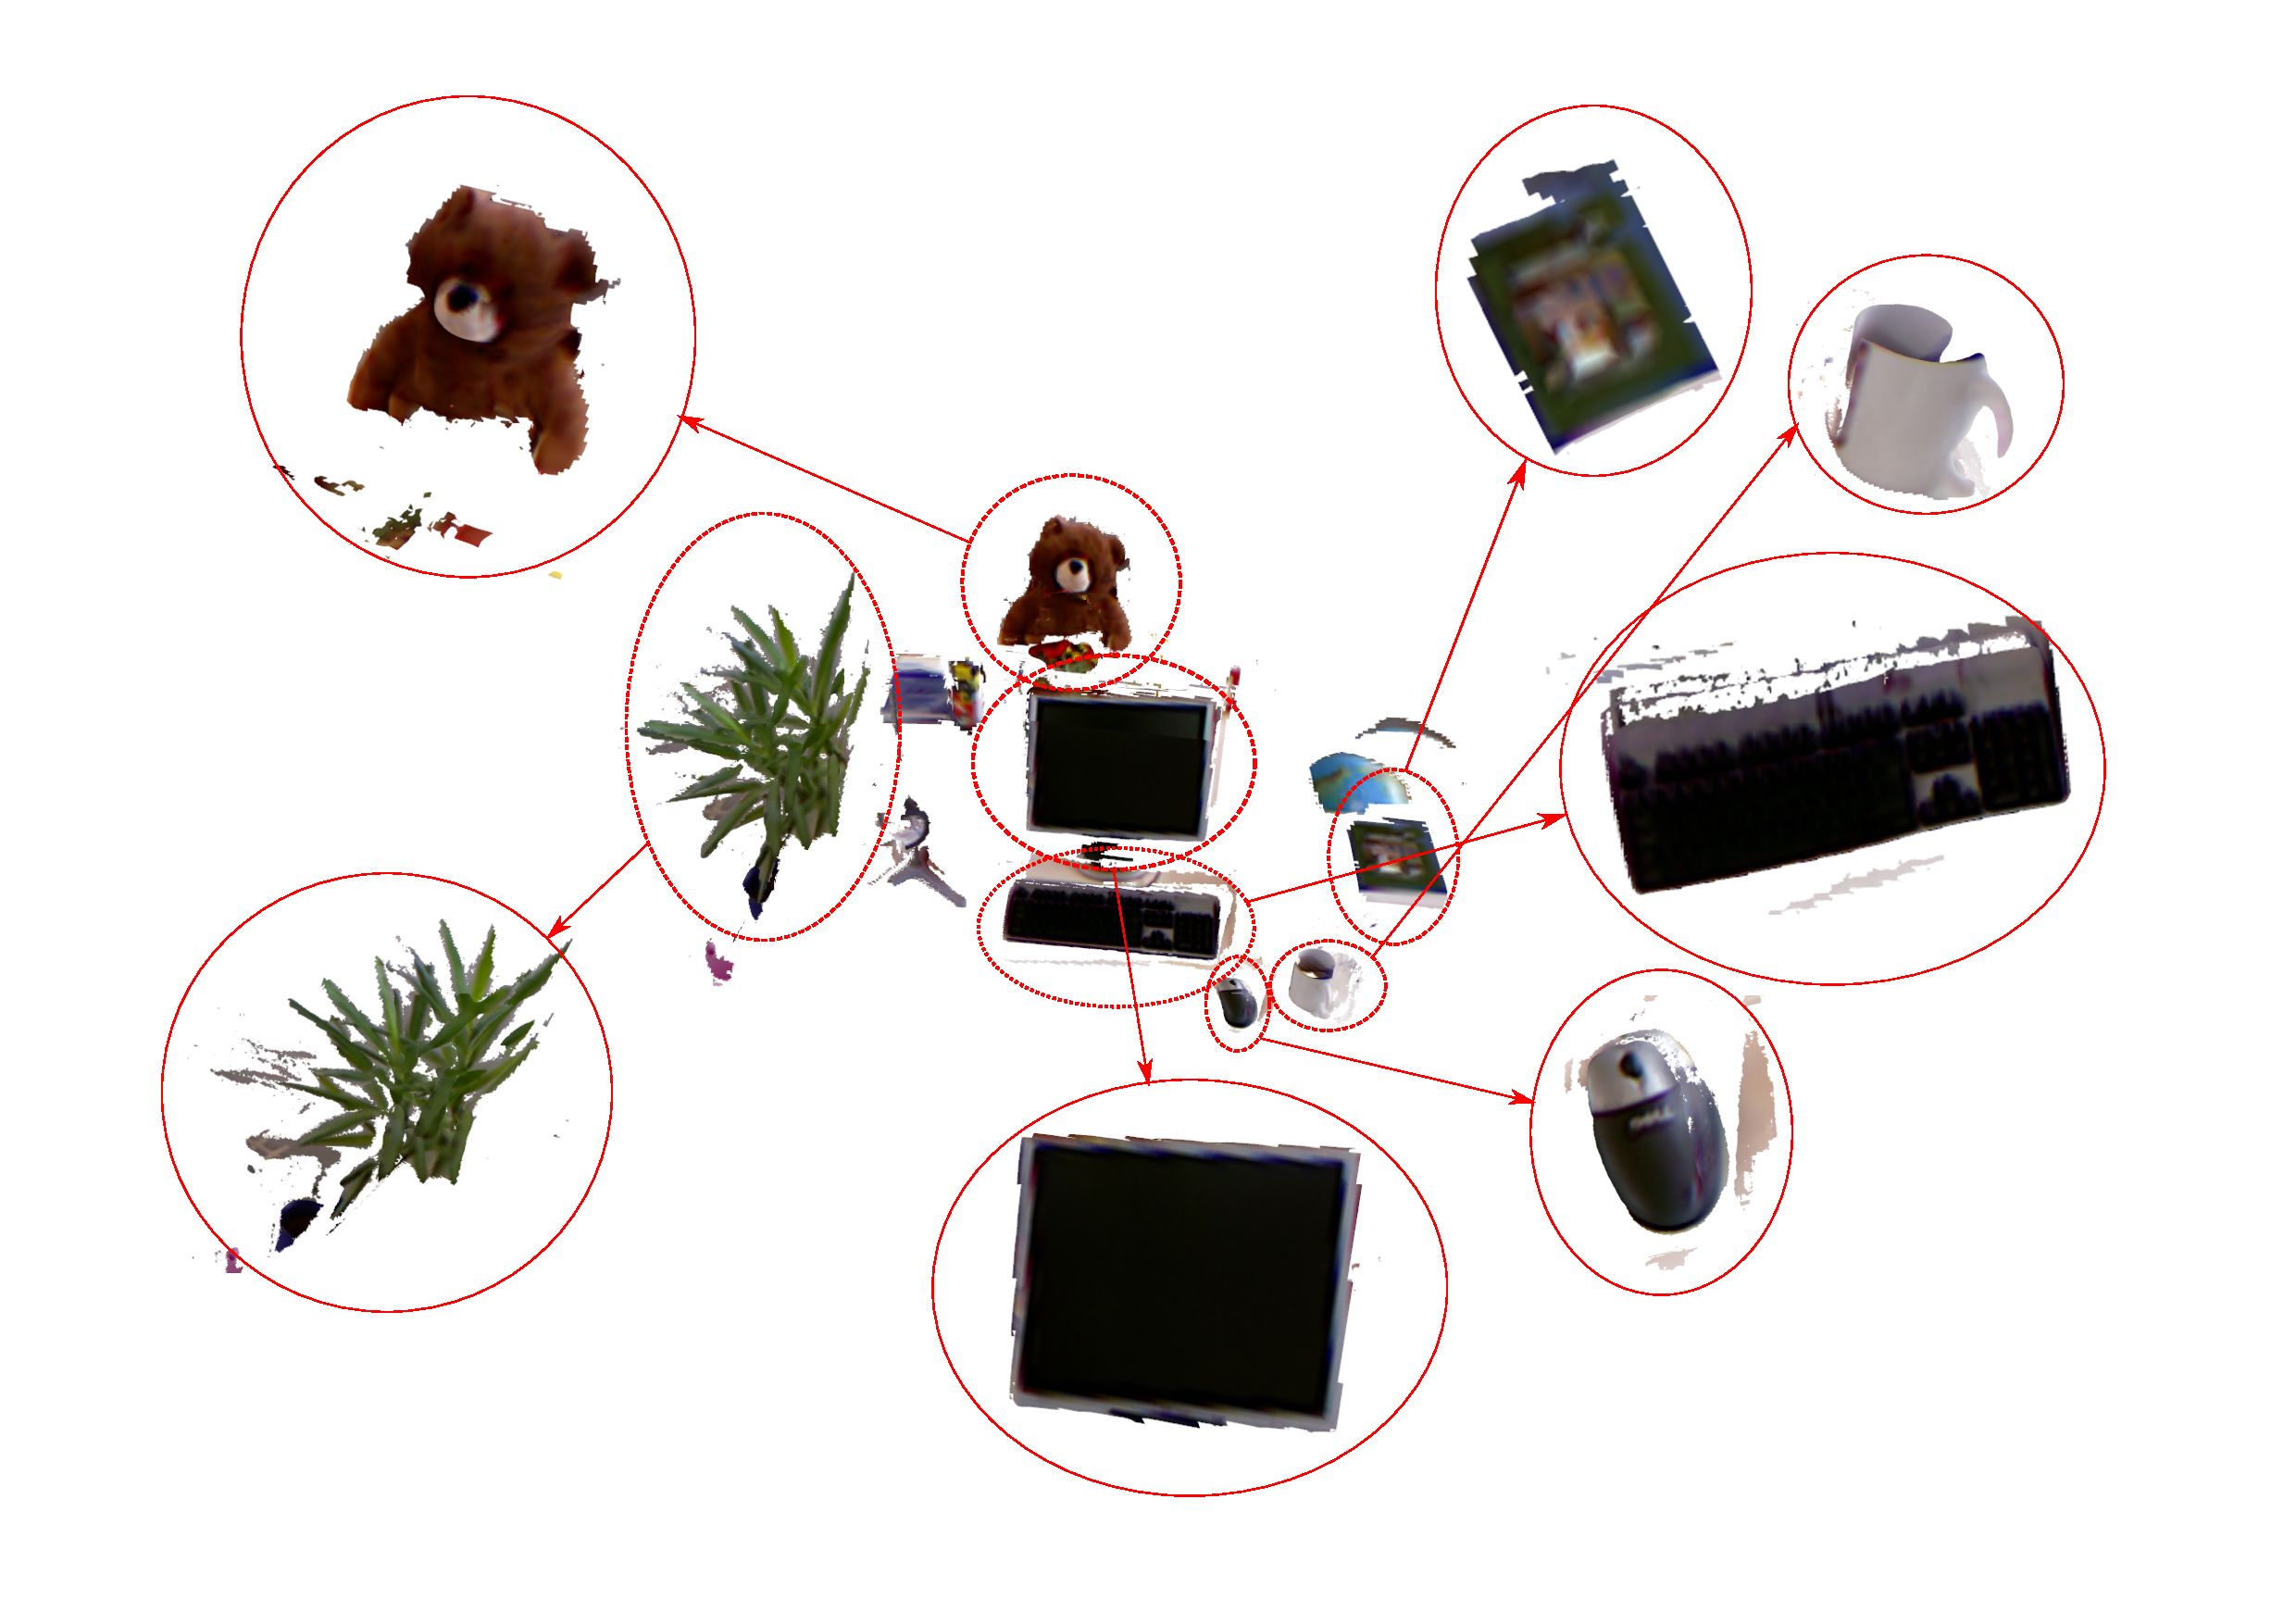
\includegraphics[width=\linewidth]{figs/teaser.pdf}\vspace{-1cm}
%    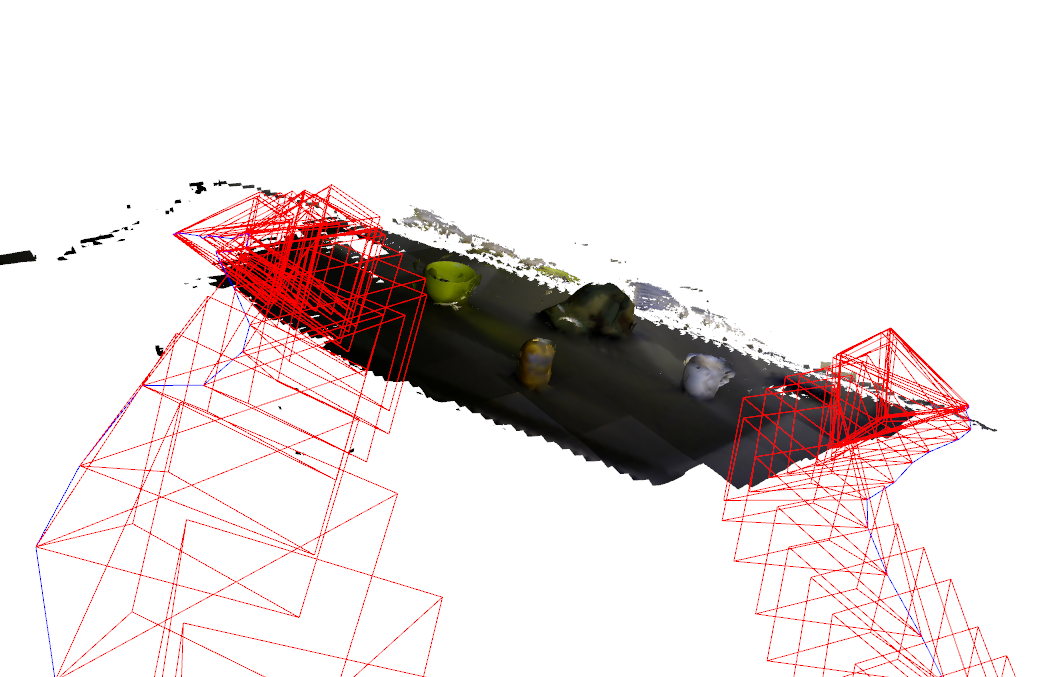
\includegraphics[width=\linewidth]{figures/scene14.png}
    \caption{Reconstruction of \textit{fr2\_xyz} sequence from \emph{tum rgbd} dataset. Our pipeline can reconstruct both camera trajectory and object models in the scene.}
    \label{fig:objectsandscene}
\end{figure}

\subsection{Contributions}

This thesis presents the following core contributions:

\begin{enumerate}
    \item A compositional volumetric rendering method that selects objects of interest and reduces memory footprint;
    \item A hybrid object association method that combines geometric and semantic cues to enable drift-free tracking without an explicit relocalization module;
    \item A scalable, modular, and easy-to-use open source system that runs nearly realtime.
\end{enumerate}

\section{Organization}

\todo{Write in the end}

